\chapter{APPLICATIONS OF SIFT-MS AND SIFDT-MS IN BREATH ANALYSIS: ANAESTHETICS}

\markboth{ANAESTHETICS IN SIFT-MS AND SIFDT-MS}{}




\section{Introduction}

\newpage
\section{Methodology}
\subsection{PTR-MS vs SIFT-MS vs SIFDT-MS}





The home-built \acrshort{sifdtms} instrument at the Heyrovsky Institute of Physical Chemistry of the Academy of Sciences in Prague (Czech Republic) has been described in detail elsewhere \cite{doi:10.1021/acs.analchem.5b02994}.

The calculation of the rate constant comes from Su \cite{su1994parametrization}

The data for $\alpha$ and $\mu_D$ can be found in \cite{lide2012crc} or in patrik's paper








\subsection{Isoflurane and sevoflurane}

\begin{figure}
  \sidesubfloat[]{\scalebox{0.7}{\begin{tikzpicture}\chemfig{[:30]F-(-[::90]F)(-[::-90]F)-(-[::60]Cl(-[::-60,2,,,white]\phantom{Cl}))(-[::-120,0.8]H)-[::-60]O-[::60](-[::60]F)-[::-60]F
  }\end{tikzpicture}}
  \label{fig:iso1}}
\qquad 
  \sidesubfloat[]{\scalebox{0.7}{\begin{tikzpicture}\chemfig{[:90]F--[::-60]O-[::60](-[::-60](-[::0]F)(-[::90]F)(-[::-90]F))(-[::60](-[::0]F)(-[::90]F)(-[::-90]F))}\end{tikzpicture}}
\label{fig:iso2}}
  \caption{Structure of (a) isoflurane and (b) sevoflurane.}
  \label{fig:iso}
\end{figure}


\subsubsection{Rate constants}

\begin{figure}%[h]
\centering
\sidesubfloat[]{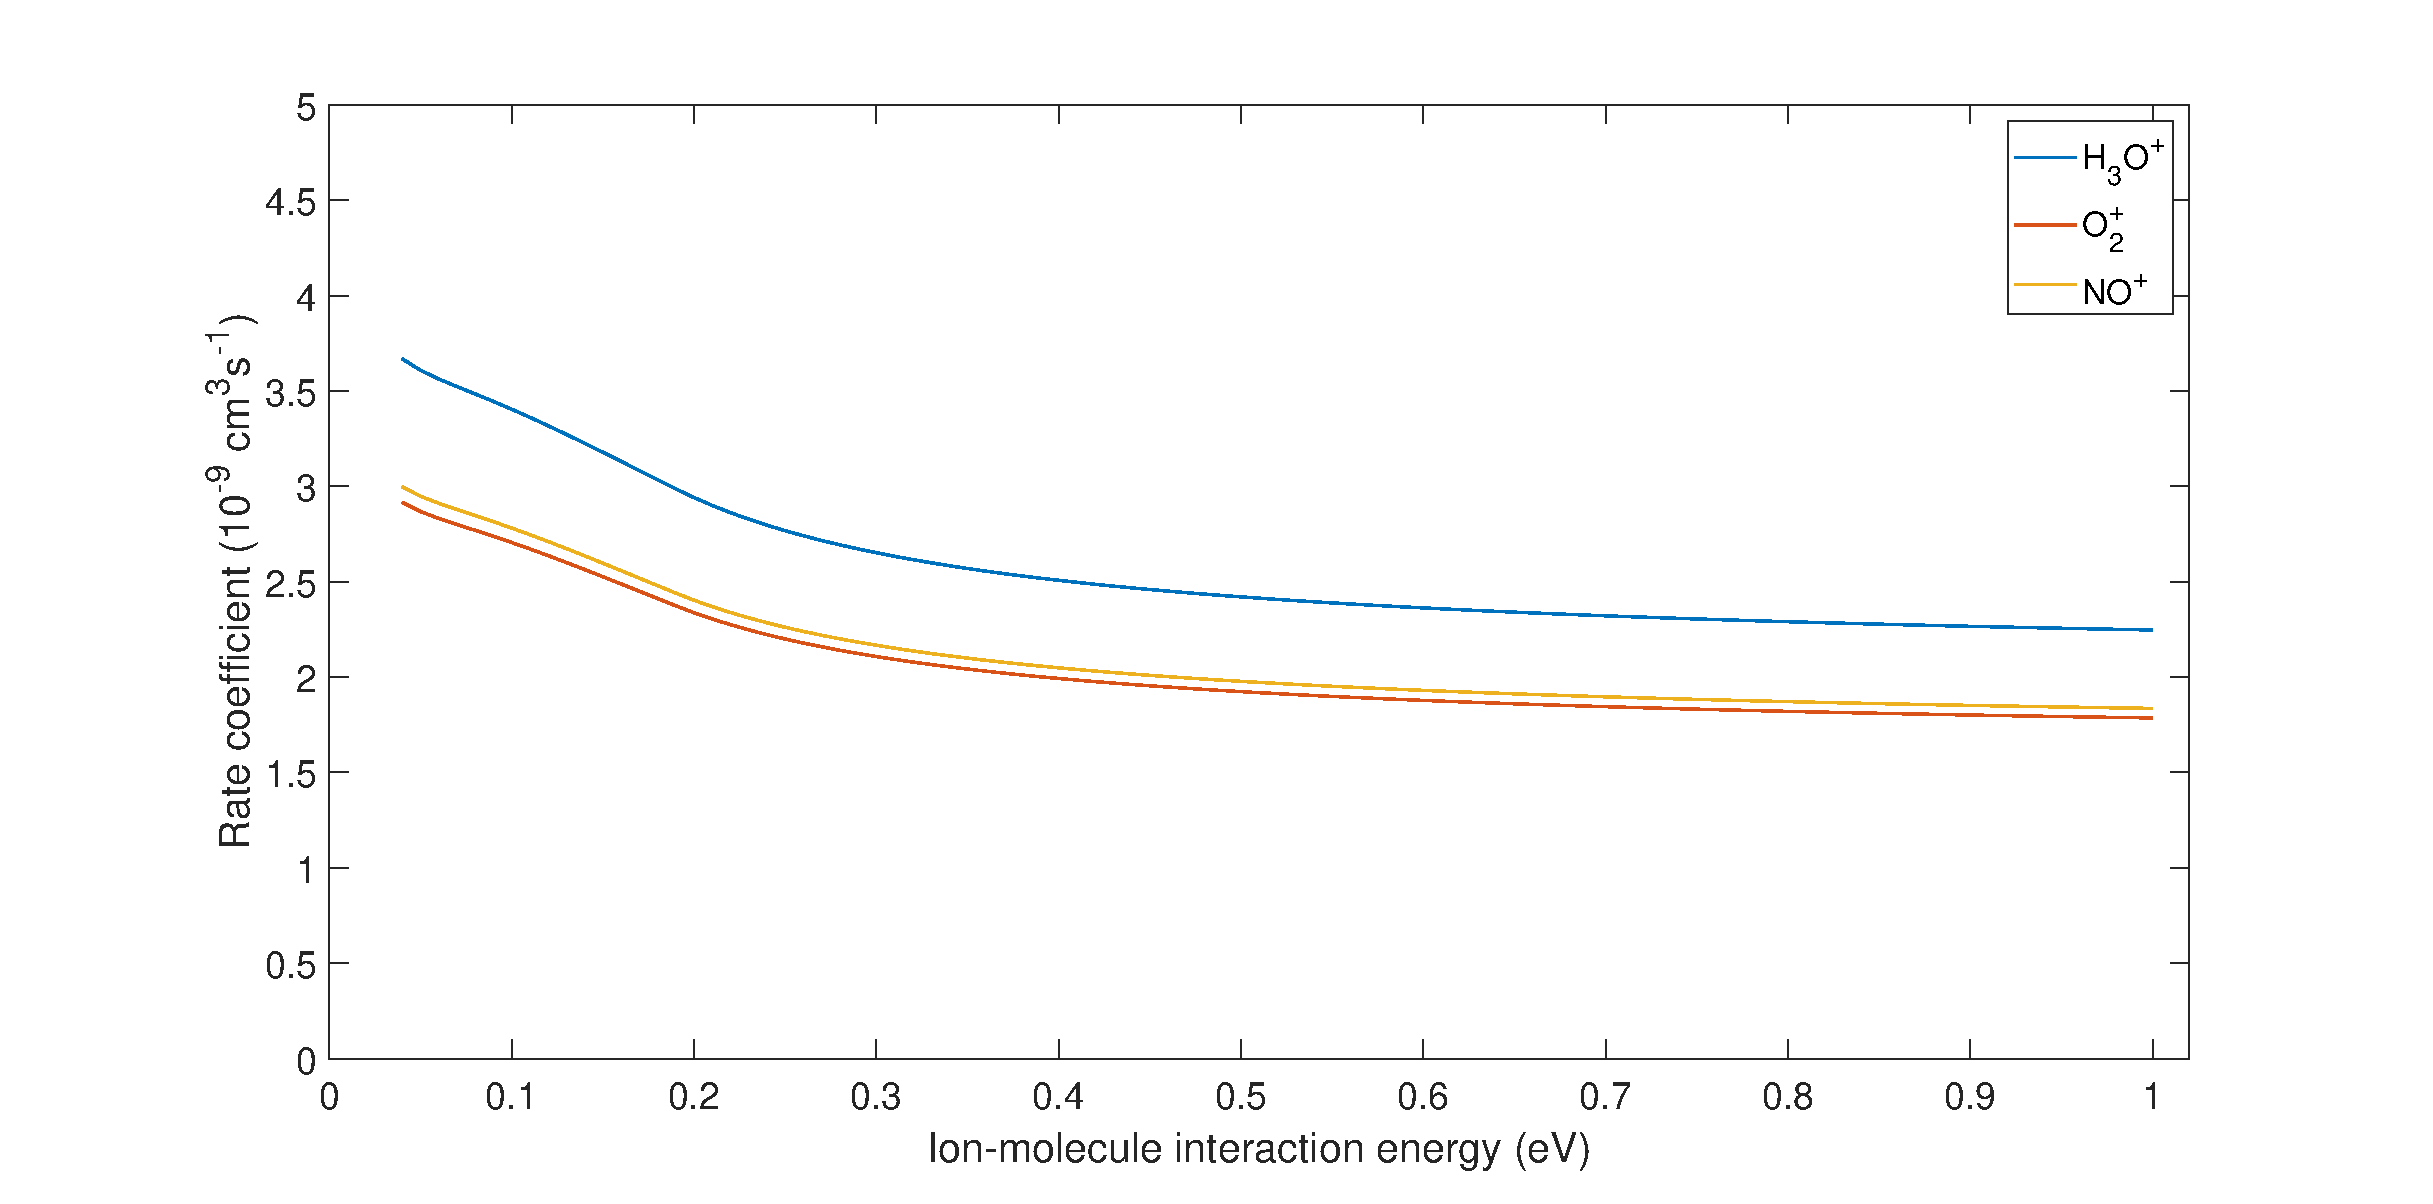
\includegraphics[width=0.9\linewidth]{pics/rate_constants_isoflurane.eps}}

\sidesubfloat[]{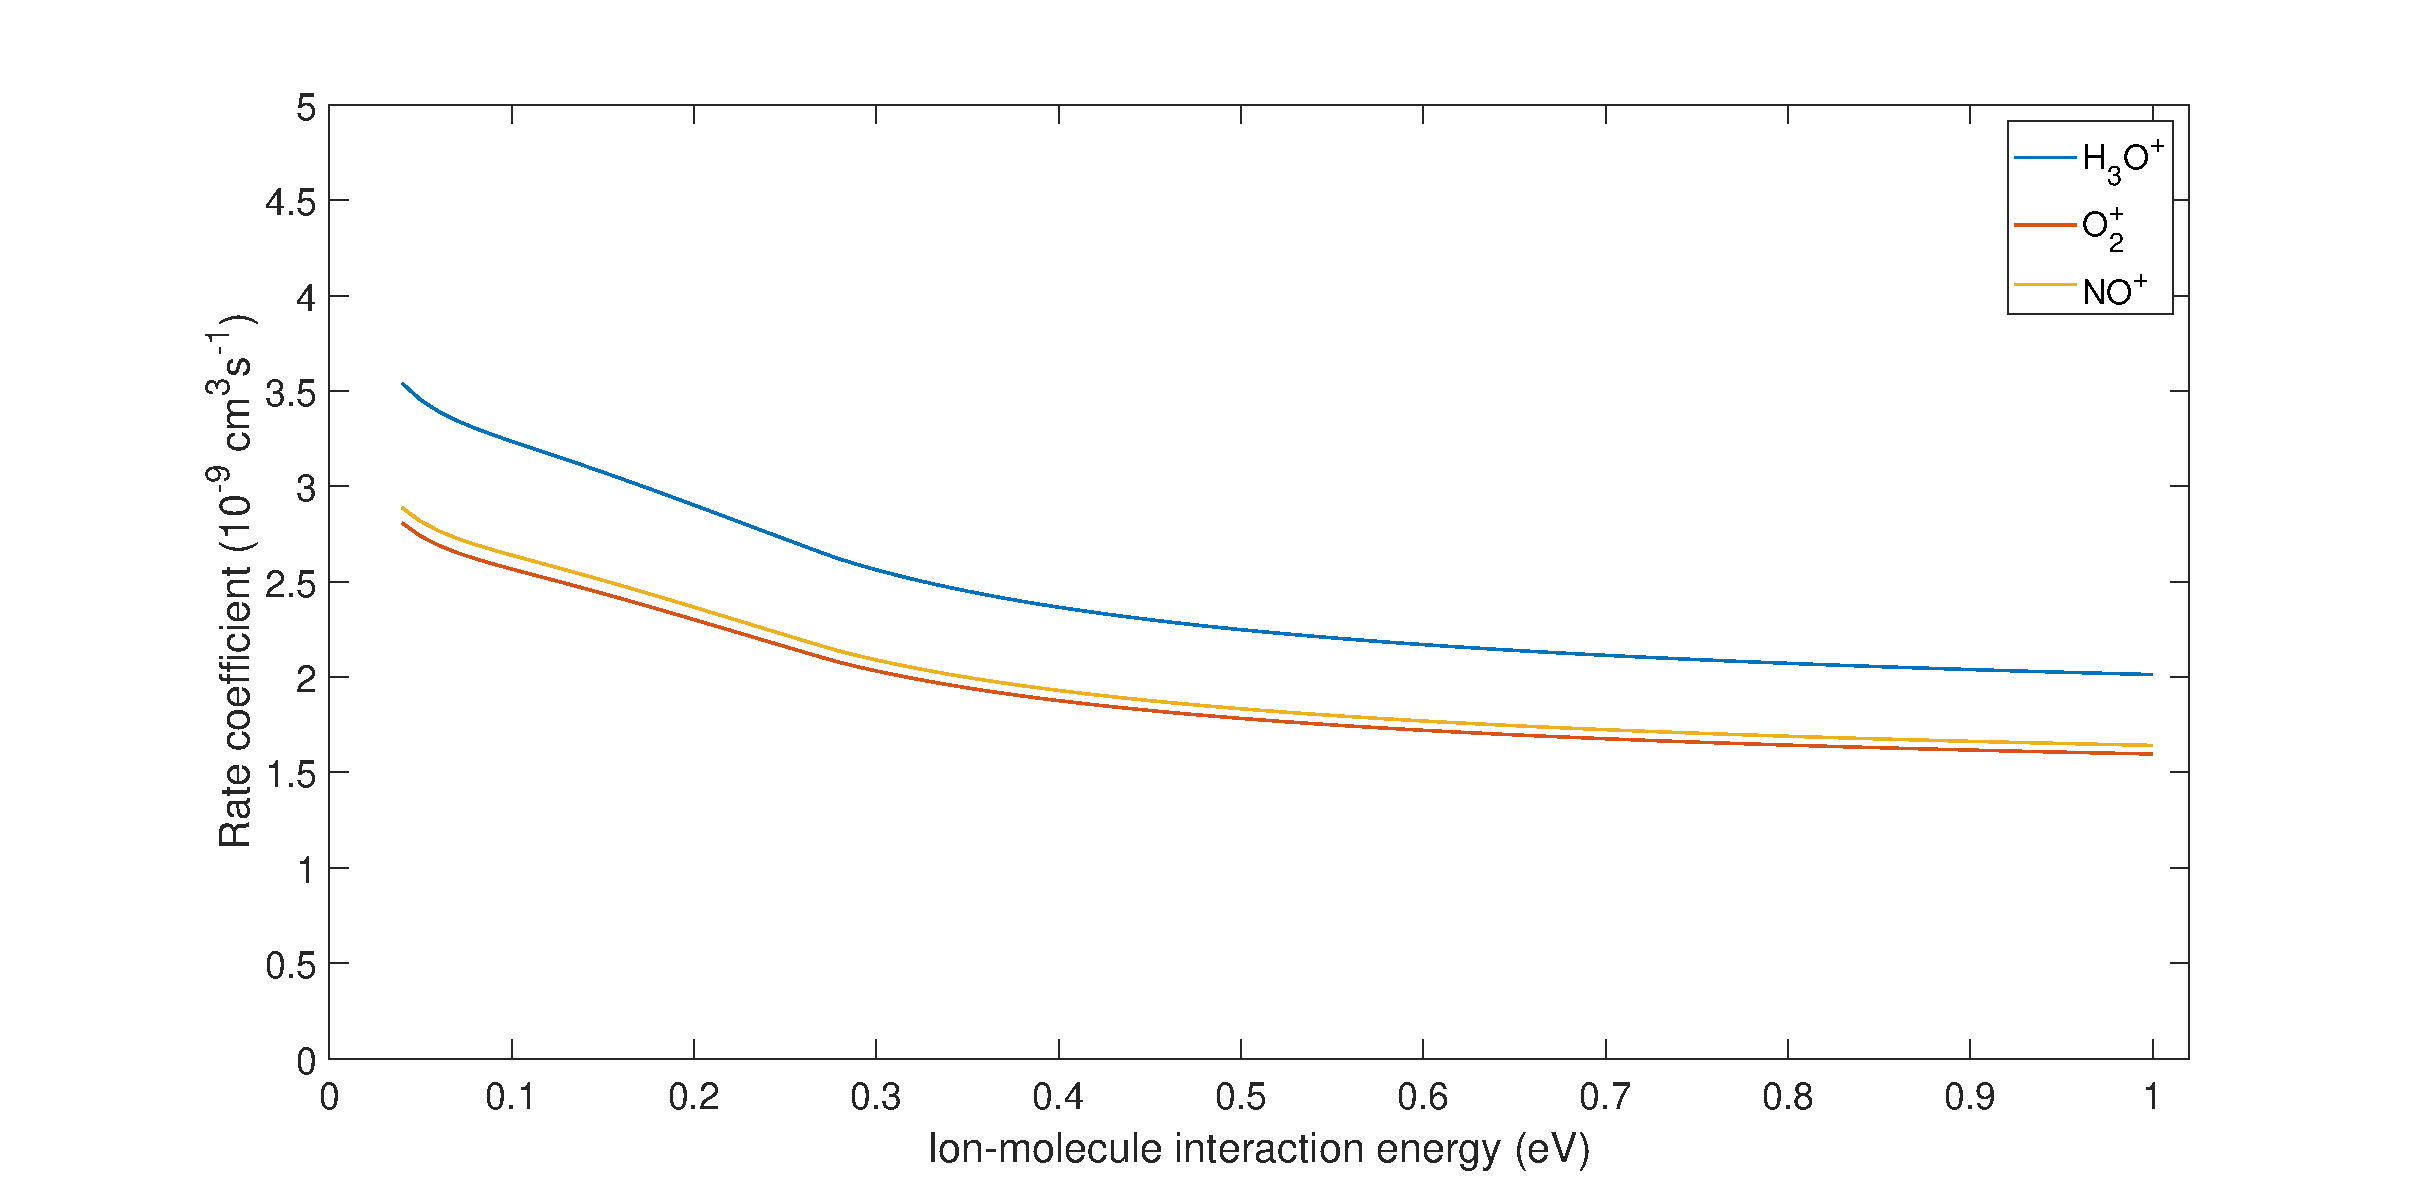
\includegraphics[width=0.9\linewidth]{pics/rate_constants_sevoflurane.eps}}
\caption{Collisional rate coefficients of (a) isoflurane and (b) sevoflurane with different reagent ions as a function of the interaction energy as predicted by the Su model \cite{su1994parametrization}}
    \label{fig:rate_iso_sevo}
\end{figure}



\section{Concerns at the moment}
There are some concerns regarding isoflurane:
\begin{itemize}
    \item It is very sensitive to humidity. In the past, people thought that the discrepancies in the PTRMS results from isoflurane measurements were due to the difference geometries of the instruments from different manufacturers, which raised doubts about the standardisation of PTRMS.
    \item There is an ion reported at m/z 163 by \cite{Wang2002SelectedSevoflurane}. The energy required for its fragmentation it is too high, around 1.8 eV.
    \item Furthermore, the ion assigned to m/z 147 does not have proper isotopic distribution (note that the scale is logarithmic and m/z 149 is not 1/3 of m/z  147)
\end{itemize}




\section{Results and discussion}
\section{Conclusions and further remarks}















